\documentclass[xcolor={dvipsnames}]{beamer}
\mode<presentation>{\usetheme{boxes}}
\usecolortheme{default}
\setbeamertemplate{navigation symbols}{}%remove navigation symbols

\setbeamerfont{frametitle}{size=\Large}

%\setbeamercolor{structure}{fg=beamer@blendedblue}



\setbeamertemplate{bibliography item}{\insertbiblabel}

\setbeamercolor{bibliography entry author}{fg=black}
\setbeamercolor{bibliography entry title}{fg=black} 
\setbeamercolor{bibliography entry location}{fg=black} 
\setbeamercolor{bibliography entry note}{fg=black}  

\usepackage[style=numeric,sorting=ydnt,maxnames=1,defernumbers=true, firstinits=true]{biblatex}
\renewbibmacro{in:}{}
\ExecuteBibliographyOptions{sorting=ydnt}

%\addbibresource{./jlescSummerSchool_checkpointing.bib}

\makeatother
\setbeamertemplate{footline}
{
  \leavevmode%
  \hbox{%
    %% \begin{beamercolorbox}[wd=.2\paperwidth,ht=2.25ex,dp=1ex]{date in head/foot}%
    %%   \usebeamerfont{date in foot}
    %% \end{beamercolorbox}%
  %%   \begin{beamercolorbox}[wd=.6\paperwidth,ht=2.25ex,dp=1ex, center]{date in head/foot}%
  %%     \usebeamerfont{date in foot}\insertshortdate
  %% \end{beamercolorbox}%
  \begin{beamercolorbox}[wd=\paperwidth,ht=2.25ex,dp=1ex]{date in head/foot}%
    \usebeamerfont{date in foot}\hfill
    {\scriptsize\insertframenumber{}}\hspace*{2ex}
  \end{beamercolorbox}}%
  \vskip0pt%
}
\makeatletter



\usepackage[utf8]{inputenc}
%\usepackage[T1]{fontenc}
%\usepackage[francais]{babel}
\usepackage{hyperref}
\usepackage{url}
\usepackage{pifont}
\usepackage{changepage}
\usepackage{listings}
\lstset{basicstyle=\ttfamily,
  showstringspaces=false,
  commentstyle=\color{black},
  keywordstyle=\color{black}
}

\usepackage{fancyvrb}
\usepackage{multirow}
\usepackage{tabu} 
\usepackage{colortbl}

\usepackage{marvosym}

\usepackage{eurosym}

%\usepackage{gitdags}
\usepackage{comment}

\usepackage{pdfpages}
\setbeamercolor{background canvas}{bg=}


\usepackage{perpage} %the perpage package
\MakePerPage{footnote}



\definecolor{beamer@blendedblue}{RGB}{0,102,204}

\definecolor{beamer@lightgray}{RGB}{238,238,224}


\definecolor{itemorange}{RGB}{255,114,0}


\definecolor{myorange}{RGB}{255,103,0}


\setbeamertemplate{itemize items}[circle]
\setbeamertemplate{itemize subitem}[triangle]


\setbeamercolor{itemize item}{fg=beamer@blendedblue}
\setbeamercolor{itemize subitem}{fg=gray}


\newcommand<>{\Blue}[1]{{\color#2{beamer@blendedblue}#1}}
%\newcommand<>{\Orange}[1]{{\color#2{BurntOrange}#1}}
\newcommand<>{\Orange}[1]{{\color#2{myorange}#1}}
\newcommand<>{\Alert}[1]{{\Orange{\textbf{#1}}}}


\newcommand{\largeskip}{\vspace{0.6cm}}
\newcommand{\hugeskip}{\vspace{1cm}}



\usepackage{tikz}
\usetikzlibrary{%
decorations.pathreplacing,%
decorations.pathmorphing,%
decorations.shapes,%
decorations.text,%
decorations.markings,%
shapes,%
shapes.callouts,%
shadows,%
arrows,
calc,%
positioning,%
chains,%
backgrounds,%
fit, %
fadings}

\tikzset{
    invisible/.style={opacity=0},
    visible on/.style={alt={#1{}{invisible}}},
    alt/.code args={<#1>#2#3}{%
      \alt<#1>{\pgfkeysalso{#2}}{\pgfkeysalso{#3}} % \pgfkeysalso doesn't change the path
    },
}


\tikzset{
    colornode/.style={
        outer sep=0pt, fill=#1!67, %text height=2ex, text depth=.5ex
    },
    cpu/.style={
        diamond, fill=gray!30, aspect=3, name=CPU#1,
        node contents={$\text{CPU}_{#1}$},
    },
    thread/.style={fill=#1!67,
        minimum width=5ex, minimum height=1.25em},
    tick/.style={very thin},
}



\newcommand{\email}[1]{\href{mailto:#1}{\nolinkurl{#1}}}

\newcommand{\xmark}{\ding{55}}


\AtBeginPart{
  %\frame{\partpage}
  \frame{
    \frametitle{Agenda}
    \small
    \tableofcontents[part=\insertpartnumber,
    sectionstyle=show,
    subsectionstyle=hide,
    subsubsectionstyle=hide]
  }
}

\AtBeginSection[]
{
  \begin{frame}
    \frametitle{Agenda}
    \small
    \tableofcontents[
    sectionstyle=show/shaded,
    subsectionstyle=show/show/hide,
    subsubsectionstyle=hide]
  \end{frame}
}

\AtBeginSubsection[]{
  \mode<presentation>{
    \frame{\tableofcontents[
      sectionstyle=show/hide,
      subsectionstyle=show/shaded/hide,
      subsubsectionstyle=show/show/hide]
    }
  }
}


\date[\the\year]{\the\year}

\newcommand{\shellcmd}[1]{\indent\indent\texttt{\footnotesize\$ #1}}


\title[]{Cloud Computing}
\subtitle{Concepts d'applications \textit{Cloud native}\footnote{Adapté du support développé par Thomas ROPARS et Renaud LACHAIZE}}

%Thomas ROPARS : \url{https://tropars.github.io/teaching/},
%\url{https://roparst.gricad-pages.univ-grenoble-alpes.fr/cloud-tutorials/m2gi-devops/}}}


\author[]{\\Danilo Carastan dos Santos
  \\ \vspace{0.5cm} \email{danilo.carastan-dos-santos@univ-grenoble-alpes.fr}}

\definecolor{mybrown}{RGB}{205,133,63}
\definecolor{myblue}{RGB}{28,134,238}

\let\Red=\alert
\newcommand<>{\green}[1]{{\color#2{green!70!black}#1}}
\newcommand<>{\blue}[1]{{\color#2{blue!100!black!100}#1}}
\definecolor{darkgreen}{rgb}{0,0.5,0}

\newcommand\myvdots{{\smash[b]\strut\smash[t]\vdots}}


\usepackage{boxedminipage}
\newenvironment{boitecode}[1]{
    \begin{boxedminipage}{\linewidth}      
%\begin{beamerboxesrounded}[shadow=true,lower=lightex,upper=medex]{#1}
    #1
    \begin{semiverbatim}
}{   \end{semiverbatim}\vspace{-1.5\baselineskip}
    \end{boxedminipage}
%  \end{beamerboxesrounded}
}


\begin{document}


\begingroup
\setbeamercolor{titlelike}{bg=beamer@lightgray, fg=black}
\begin{frame}
\titlepage
\end{frame}
\endgroup

\begin{frame}
  \frametitle{Motivation : du data-centre privé (\textit{on premises}) au Cloud}
  \begin{columns}
    \begin{column}{.5\linewidth}
      \begin{itemize}
        \item Migration d'applications existantes
        \item \textit{``Lift and Shift''} : Réhébergement entier de l'application vers un Cloud public ou privé
        \item Migration via IaaS ou PaaS
      \end{itemize}
      
    \end{column}
    \begin{column}{.5\linewidth}
      \centering 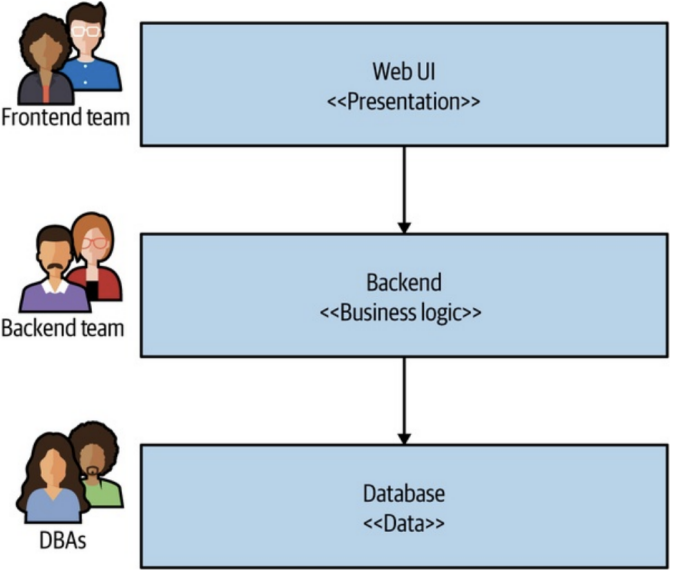
\includegraphics[width=\linewidth]{Figures/3-tier-app.png}  
    \end{column}
  \end{columns}
\vspace{5mm}

 \textbf{Tendence : } Concevoir de nouvelles applications en prenant en compte
    dès le départ les spécificités (défis et opportunités) des plateformes et
    technologies Cloud modernes

\end{frame}

\begin{frame}
  \frametitle{\textit{Cloud Native}}
  \begin{block}{Une définition\footnote{\url{https://github.com/cncf/toc/blob/main/DEFINITION.md\#fran\%C3\%A7ais}}}
    \begin{footnotesize}
      ``\textbf{Les technologies Cloud Native permettent aux entreprises de construire et
      d'exploiter des applications élastiques dans des environnements modernes
      et dynamiques comme des clouds publics, privés ou bien hybrides.} Les
      conteneurs, le maillage de services, les microservices, les
      infrastructures immuables et les API déclaratives illustrent cette
      approche.

\textbf{Ces techniques permettent la mise en œuvre de systèmes faiblement couplés, à la
fois résistants, pilotables et observables.} Combinés à un r\textbf{obuste système
d'automatisation}, ils permettent aux ingénieurs de \textbf{procéder à des modifications
impactantes, fréquemment et de façon prévisible} avec un minimum de travail.

La Cloud Native Computing Foundation cherche à favoriser l'adoption de ce
paradigme en encourageant et en soutenant un écosystème de projets open source
et indépendants. Nous démocratisons l'état de l'art des bonnes pratiques afin de
rendre l'innovation accessible à tous.''
    \end{footnotesize}
    
  \end{block}
\end{frame}

\begin{frame}
  \frametitle{\textit{Cloud Native}}

  \begin{block}{Une autre définition\footnote{J. Garrisson and K. Nova. Cloud native infrastructure. O’Reilly, 2017.}}
    \begin{normalsize}
      \textit{``A cloud native application is engineered to run on a platform and is designed for resiliency, agility,
      operability, and observability.''}
    \end{normalsize}
    
  \end{block}

  \begin{itemize}
    \item \textbf{Résilience :} Profiter de la nature dynamique et distribuée du Cloud
    pour s'adapter et rester opérationnelle face à des pannes
    \item \textbf{Agilité :} permettre des déploiements et des interactions rapides
    \item \textbf{Opérabilité :} ajouter le contrôle des cycles de vie des applications
    depuis l'intérieur de l'application au lieu de s'appuyer sur des processus
    et des moniteurs externes
    \item \textbf{Observabilité :} fournir des informations pour répondre aux questions
    sur l'état de l'application
  \end{itemize}  
\end{frame}


\begin{frame}
  \frametitle{Transition vers le \textit{Cloud Native} : un exemple}
  \noindent + Niveau faible, moyen et élevé de sous-traitance de responsabilités\\ 
  + Réduction de coûts litées à la gestion d'infrastructure physique/logiciel\\
  + Niveau faible, moyen et élevé de dépendance d'un fournisseur de Cloud  

\vspace{5mm}
  \centering 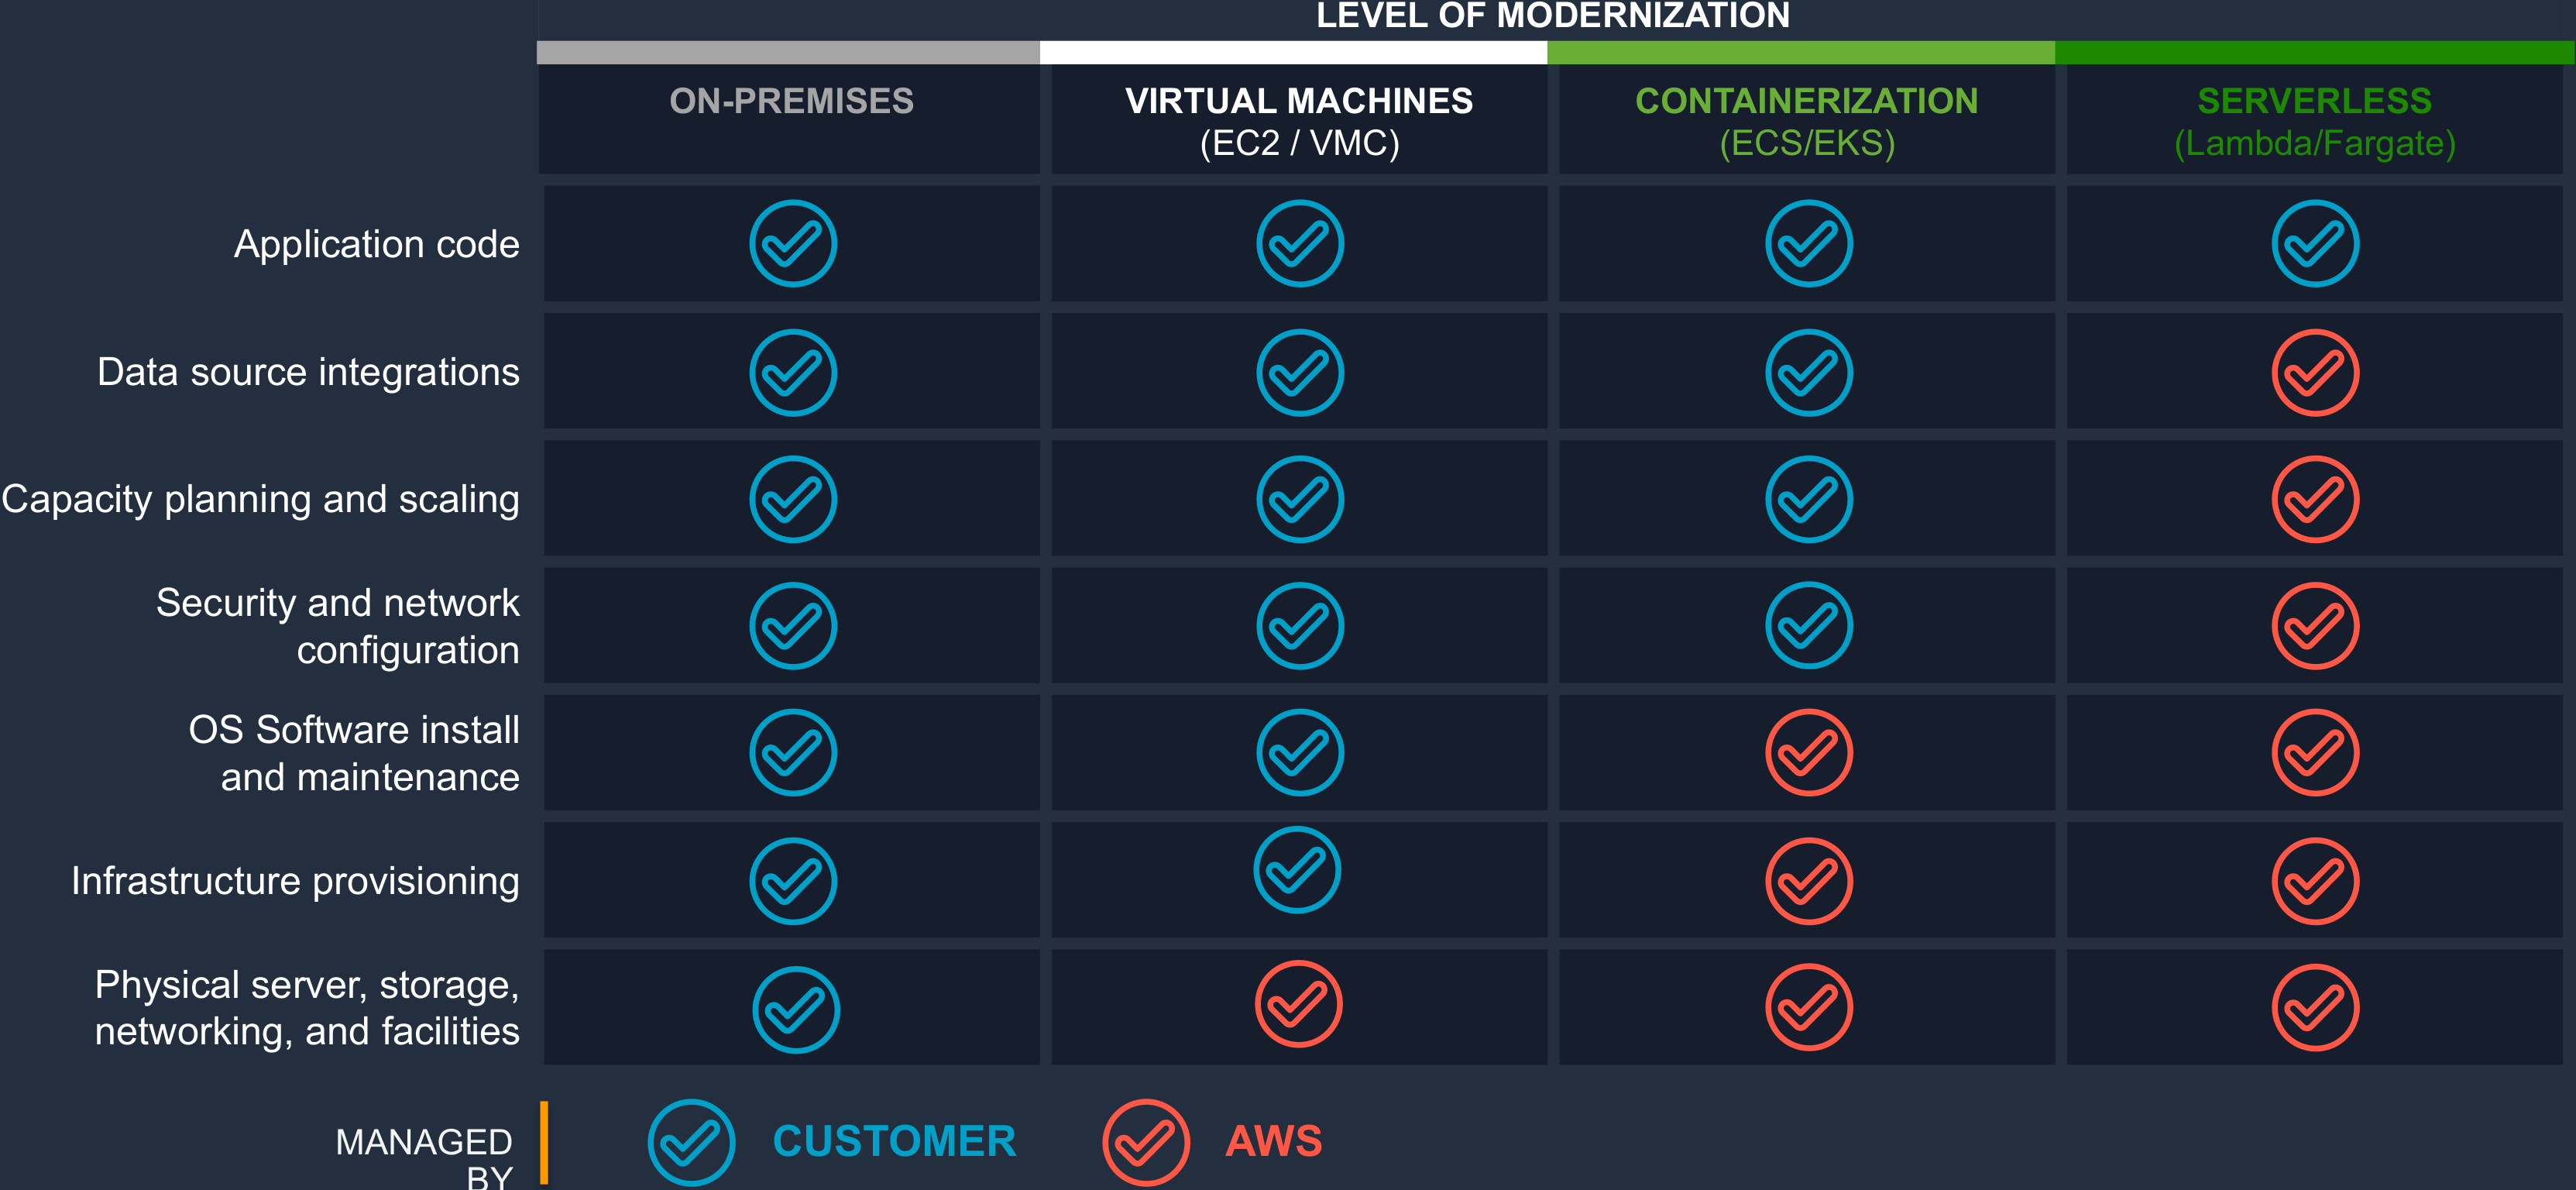
\includegraphics[width=\linewidth]{Figures/cloud-native-aws.png} 
\end{frame}


\begin{frame}
  \frametitle{Quelques méthodologies liées}

  \begin{itemize}
    \item Conteneurs, CI/CD, \textbf{Microservices}, \textit{Serverless} (FaaS)
  \end{itemize}  

\end{frame}

\begin{frame}
  \frametitle{Architecture monolithique à 3 niveaux}
  \begin{columns}
    \begin{column}{.5\linewidth}
      \centering \noindent \textit{Backend} monolithique
      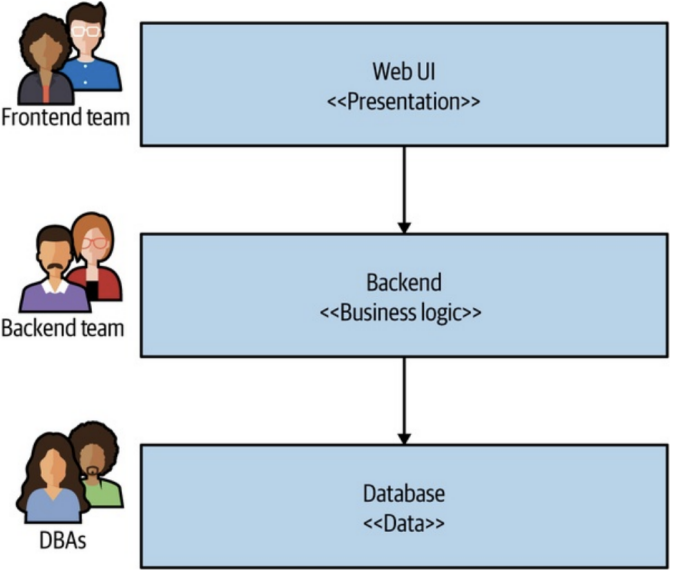
\includegraphics[width=\linewidth]{Figures/3-tier-app.png}      
    \end{column}
    \begin{column}{.5\linewidth}
      \noindent Un niveau monolithique
      \centering 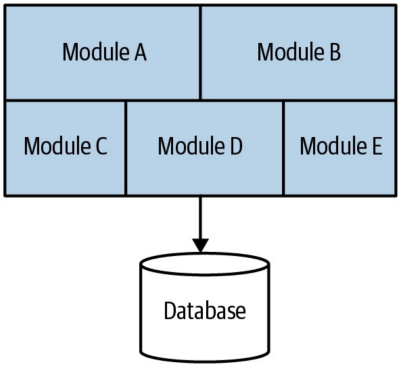
\includegraphics[width=.8\linewidth]{Figures/monolith.png}     
    \end{column}
  \end{columns}
\end{frame}

\begin{frame}
  \frametitle{Monolithe modulaire}
  \begin{columns}
    \begin{column}{.4\linewidth}
      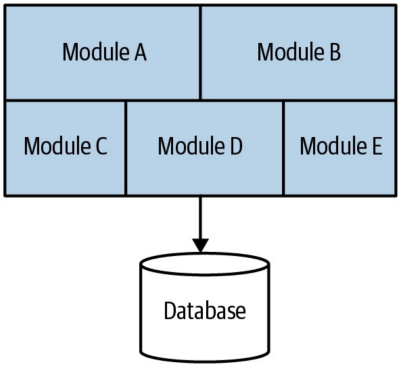
\includegraphics[width=\linewidth]{Figures/monolith.png}      
    \end{column}
    \begin{column}{.6\linewidth}
      \begin{itemize}
        \item Modulaire mais typiquement déployé comme un processus unique (monolithique)
        \item Problèmes liés :
        \begin{itemize}
          \item Qui décide sur quoi ? Qui détient quoi ?
          \item Pas d'indépendance pour mettre à jour un module
        \end{itemize}
      \end{itemize}   
    \end{column}
  \end{columns}
\end{frame}

\begin{frame}
  \frametitle{Microservices\footnote{Source de la figure : \url{https://github.com/delimitrou/DeathStarBench/tree/master/socialNetwork}}}
  \centering 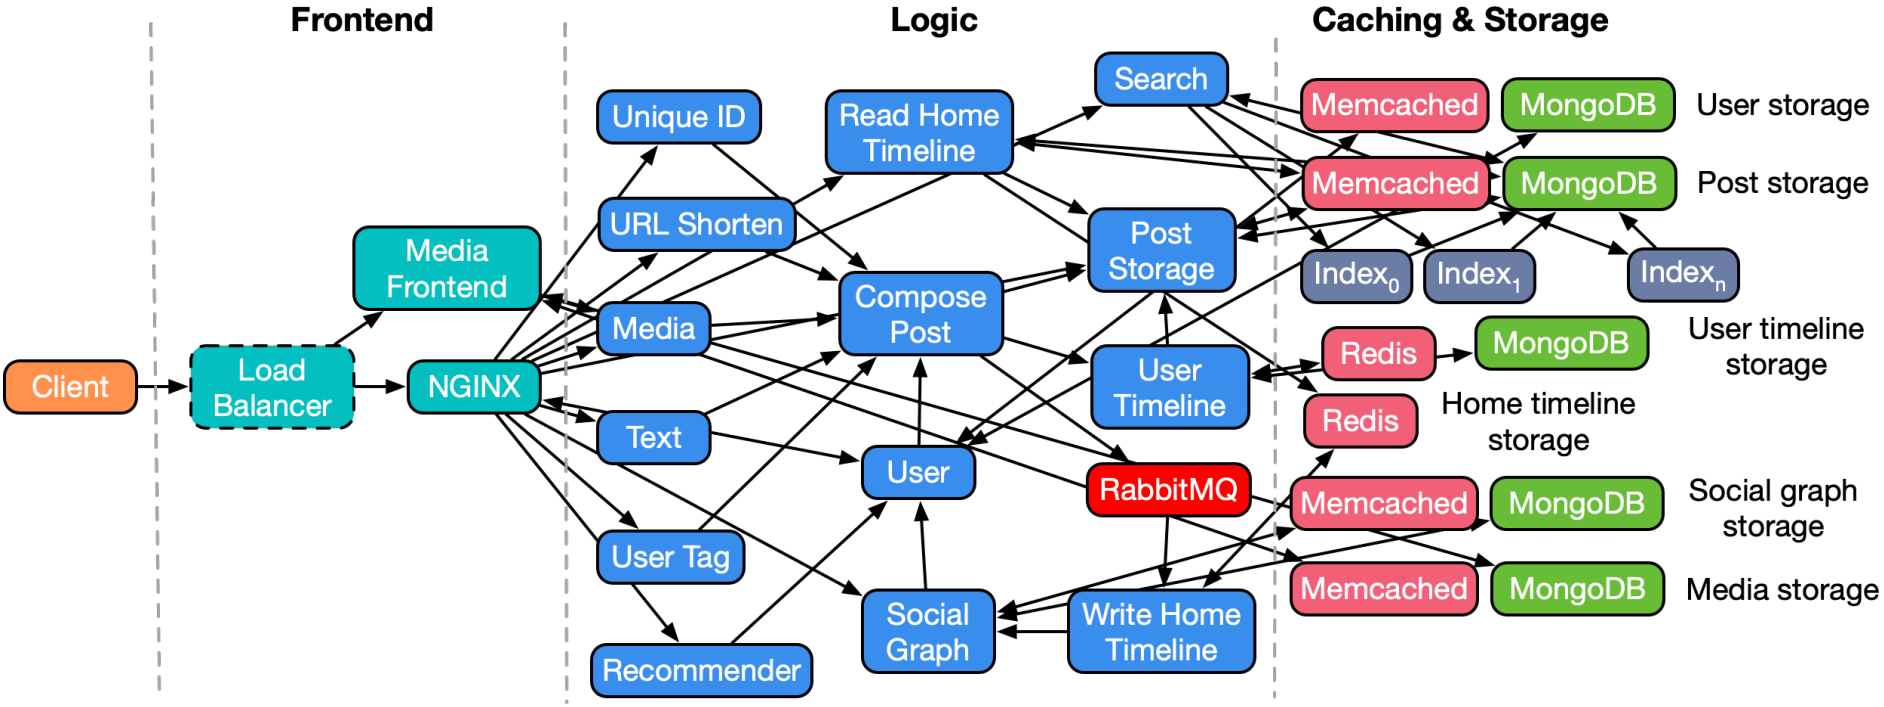
\includegraphics[width=\linewidth]{Figures/microservices-general.png}
  
  \begin{itemize}
    \item Déployer les modules de façon indépendante
    \item Posséder l'état de chaque module
    \item Aligner sur l'organisation et structure de l'activité de l'entreprise
  \end{itemize}

\end{frame}

\begin{frame}
  \frametitle{Objectives}
  Déployer les modules de façon indépendante : 
  \begin{itemize}
    \item Modifier un service sans modifier les autres services
    \item Réduire le temps de déploiement de nouvelles fonctionnalités
  \end{itemize}
  Posséder l'état de chaque module : 
  \begin{itemize}
    \item Éviter utiliser de bases de données partagées
  \end{itemize}
\end{frame}

\begin{frame}
  \frametitle{Aligner sur l'organisation et structure de l'activité de l'entreprise}
  

  \begin{block}{Loi de Conway (\textit{Conway's law})\footnote{\url{https://martinfowler.com/bliki/ConwaysLaw.html}} :} 
    
    \textit{Any organization that designs a system (defined broadly) will produce a
    design whose structure is a copy of the organization's communication
    structure.}

  \end{block}

  \textbf{Conséquences : }
  \pause

  \begin{itemize}
    \item Un petit groupe de développeurs qui travaillent dans le même bureau $\rightarrow$ vont produire un monolithe
    \item Organisation basée sur une expertise précise $\rightarrow$ vont produire une architecture à trois niveaux
  \end{itemize}

  Une architecture qui n'est pas alignée sur l'organisation des collaborateurs peut être contre productive
  \begin{itemize}
    \item Surcharge de communication
    \item Tension
  \end{itemize}
\end{frame}

\begin{frame}
  \frametitle{Exemple}
  \begin{columns}
    \begin{column}{.5\linewidth}
      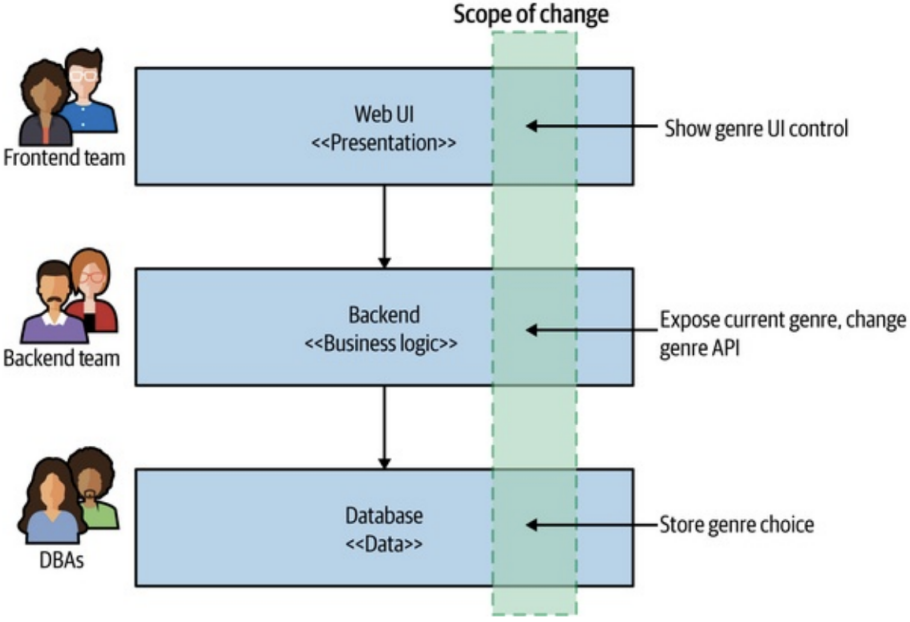
\includegraphics[width=1.2\linewidth]{Figures/microservice-example-1.png}      
    \end{column}
    \begin{column}{.5\linewidth}
      \begin{itemize}
        \item Objectif : développer un service de \textit{streaming} de musique
        \item Nous voulons ajouter une nouvelle fonctionnalité : chaque client
        pourra définir son genre de musique préféré dans son profil. 
        \begin{itemize}
          \item Plusieurs équipes doivent être impliquées
          \item Modifications doivent être déployées dans le bon ordre
        \end{itemize}
      \end{itemize}   
    \end{column}
  \end{columns}
\end{frame}


\begin{frame}
  \frametitle{Structuration par microservices}
  \begin{itemize}
    \item Délimiter les frontières de microservices en fonction du domaine d'activité
    \item Inspiré par l'approche \textit{Domain-Driven Design}
  \end{itemize}

  \vspace{10mm}

  \centering 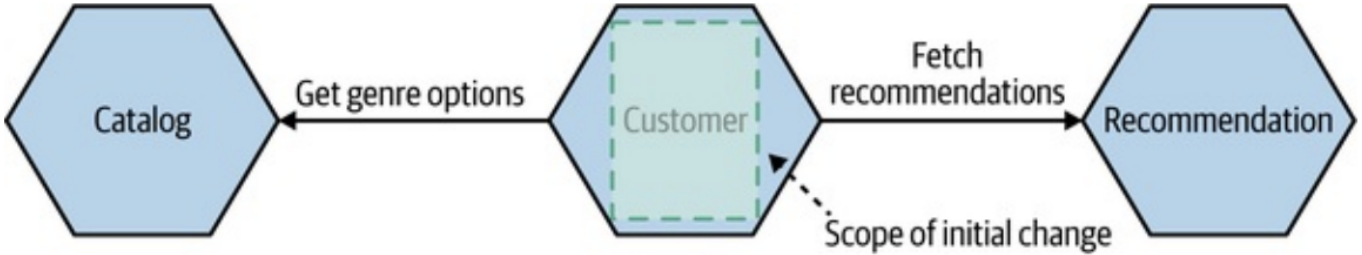
\includegraphics[width=1\linewidth]{Figures/microservice-example-2.png}  

\end{frame}

\begin{frame}
  \frametitle{Structuration par microservices}
  \begin{columns}
    \begin{column}{.5\linewidth}
      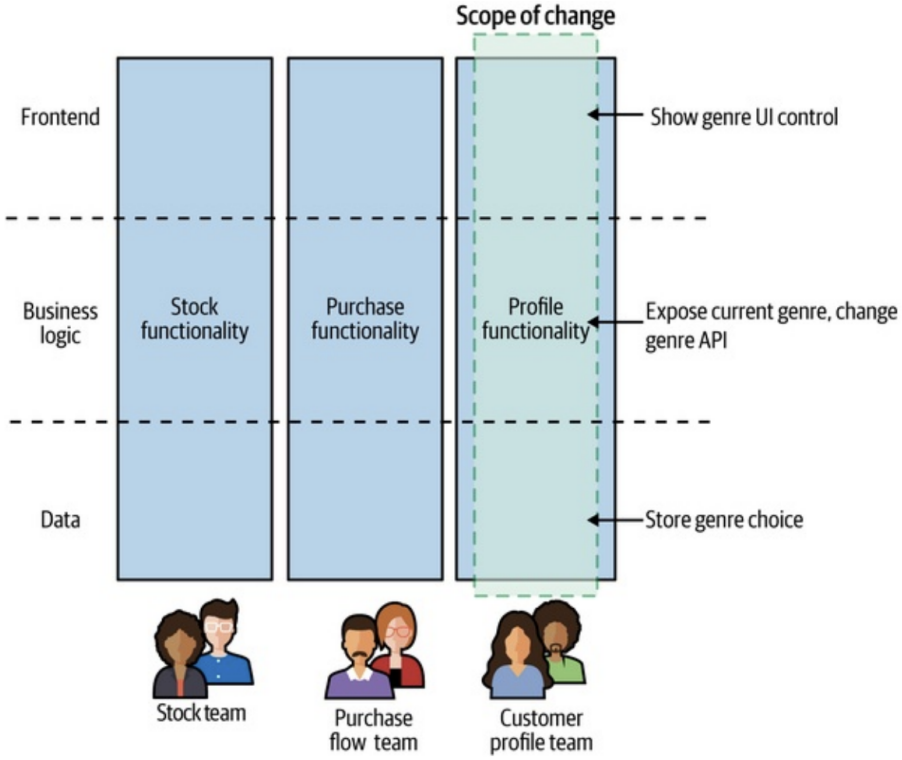
\includegraphics[width=1.2\linewidth]{Figures/microservice-example-3.png}      
    \end{column}
    \begin{column}{.5\linewidth}
      \begin{itemize}
        \item Une petite équipe est chargée de la fonctionnalité
        \textit{Profile}
        \item Cette équipe comprend des développeurs frontend, backend et de
        base de données 
        \item Nouvelle organisation :
        \begin{itemize}
          \item Petite équipe polyvalente (de 5 à 10 personnes)
          \item Objectif : Faciliter les interactions entre les équipes et leurs
          membres          
        \end{itemize}
      \end{itemize}   
    \end{column}
  \end{columns} 
\end{frame}

\begin{frame}{Technologies liées aux microservices}{Communication}
  
  Communication synchrone et bloquante :
  \begin{itemize}
    \item \textit{Remote Procedure Calls} : gRPC\footnote{\url{https://grpc.io/}}
    \item REST\footnote{\url{https://www.redhat.com/fr/topics/api/what-is-a-rest-api}} + HTTP
  \end{itemize}
  
  Communication non bloquante par queues/événements/producteur-consommateur :
  \begin{itemize}
    \item Kafka\footnote{\url{https://kafka.apache.org/}}, RabbitMQ\footnote{\url{https://www.rabbitmq.com/}}, ZeroMQ\footnote{\url{https://zeromq.org/}}
  \end{itemize}

\end{frame}

\begin{frame}{Technologies liées aux microservices}{Déploiement}
  Conteneurs + orchestration (gestion)
  \begin{itemize}
    \item Docker\footnote{\url{https://www.docker.com/}} (conteneurs)
    \item Kubernetes\footnote{\url{https://kubernetes.io/}}, Docker Swarm\footnote{\url{https://docs.docker.com/engine/swarm/}} (orchestration)
  \end{itemize}

  Services fournis par les fournisseurs de Cloud :
  \begin{itemize}
    \item ECS/EKS (AWS)
    \item Cloud Run, Kubernetes Engine (Google)
  \end{itemize}
\end{frame}




\begin{frame}
  \frametitle{Microservices : Avantages}

  \begin{itemize}
    \item Hétérogénéité technologique
    \item Robustesse
    \item Scalabilité
    \item Facilité de déploiement
  \end{itemize} 

\end{frame}

\begin{frame}{Microservices : Avantages}{Hétérogénéité technologique}

  \begin{itemize}
    \item Possible implémentation en plusieurs langages/technologies/base de données
    \begin{itemize}
      \item Les détails internes sont cachées. Il suffit de bien communiquer
      avec les autres services
    \end{itemize}
    \item Cela s'aligne sur :
    \begin{itemize}
      \item Une équipe par microservice
      \item Une gestion décentralisée
    \end{itemize}

  \end{itemize}

  %\vspace{5mm}

  \centering 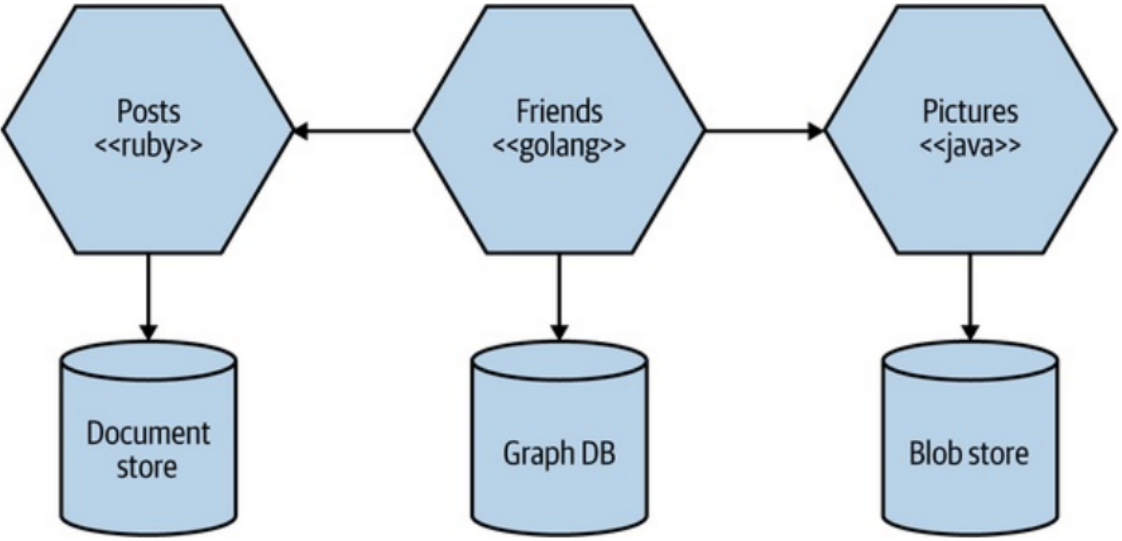
\includegraphics[width=.8\linewidth]{Figures/microservice-advantage-1.png}  
  
\end{frame}

\begin{frame}{Microservices : Avantages}{Robustesse}
  \begin{itemize}
    \item Un microservice tombe en panne != l'application tombe en panne
    \begin{itemize}
      \item Certaines parties de l'application peuvent continuer à fonctionner même lorsque certains composants tombent en panne
      \item Nécessite une bonne isolation entre les composants
    \end{itemize}
    \item Attention : de nouveaux types de pannes peuvent apparaître
  \begin{itemize}
    \item Pannes réseau
  \end{itemize}
  \end{itemize}
\end{frame}

\begin{frame}{Microservices : Avantages}{Scalabilité}

  \begin{itemize}
    \item Plusieurs instances d'un microservice peut être créées
    
    \item Cela s'aligne sur :
    \begin{itemize}
      \item Agilité : S'adapter en fonction des fluctuations de la charge de travail
      \item Résilience : Distribuer les fonctionnalités géographiquement
    \end{itemize}

  \end{itemize}

  %\vspace{5mm}

  \centering 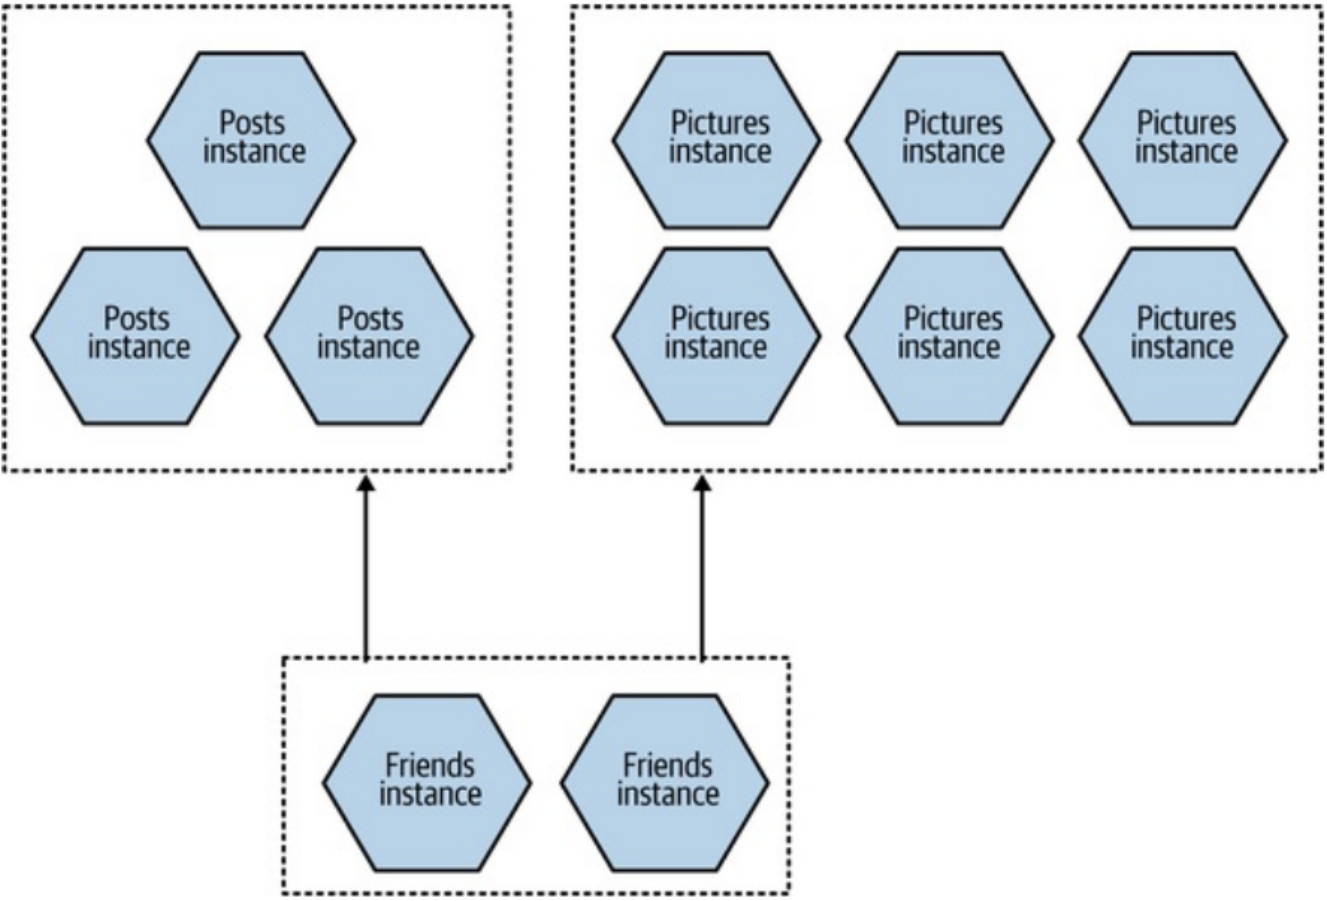
\includegraphics[width=.7\linewidth]{Figures/microservice-advantage-2.png}  
  
\end{frame}

\begin{frame}{Microservices : Avantages}{Facilité de déploiement}

  \begin{itemize}
    \item Chaque microservice peut être déployé indépendamment
    \item Il est important pour :
    \begin{itemize}
      \item Décentraliser la gestion
      \item Mettre en place de nouvelles fonctionnalités le plus rapidement possible
      (agilité)
      \item Pouvoir appliquer les approches DevOps :
      \begin{itemize}
        \item Intégration continue
        \item Livraison continue
      \end{itemize}
    \end{itemize}
  \end{itemize}
\end{frame}


\begin{frame}{Microservices : Inconvénients}
  \textbf{Développement et maintenance complexes :}
  \begin{itemize}
    \item Hétérogénéité de technologies
    \item Relations complexes entre les services
    \begin{itemize}
      \item Débogage difficile 
    \end{itemize}
    \item Difficultés liés aux bases de données distribuées 
    \begin{itemize}
      \item Gestion de l'état de l'application 
    \end{itemize}
    \item Déploiement complexe avec un grand nombre de services
    \begin{itemize}
      \item Monitoring difficile
    \end{itemize}
  \end{itemize}

  \textbf{Nécessite des développeurs expérimentés :}
  \begin{itemize}
    \item Une application monolithique peut être une solution plus appropriée
    dans certaines situations
  \end{itemize}
\end{frame}

\begin{frame}{Microservices : Inconvénients\footnote{Source de la figure : Gan,
  Yu, et al. "An open-source benchmark suite for microservices and their
  hardware-software implications for cloud \& edge systems.", ASPLOS 2019.}}
  \begin{columns}
    \begin{column}{.5\linewidth}
      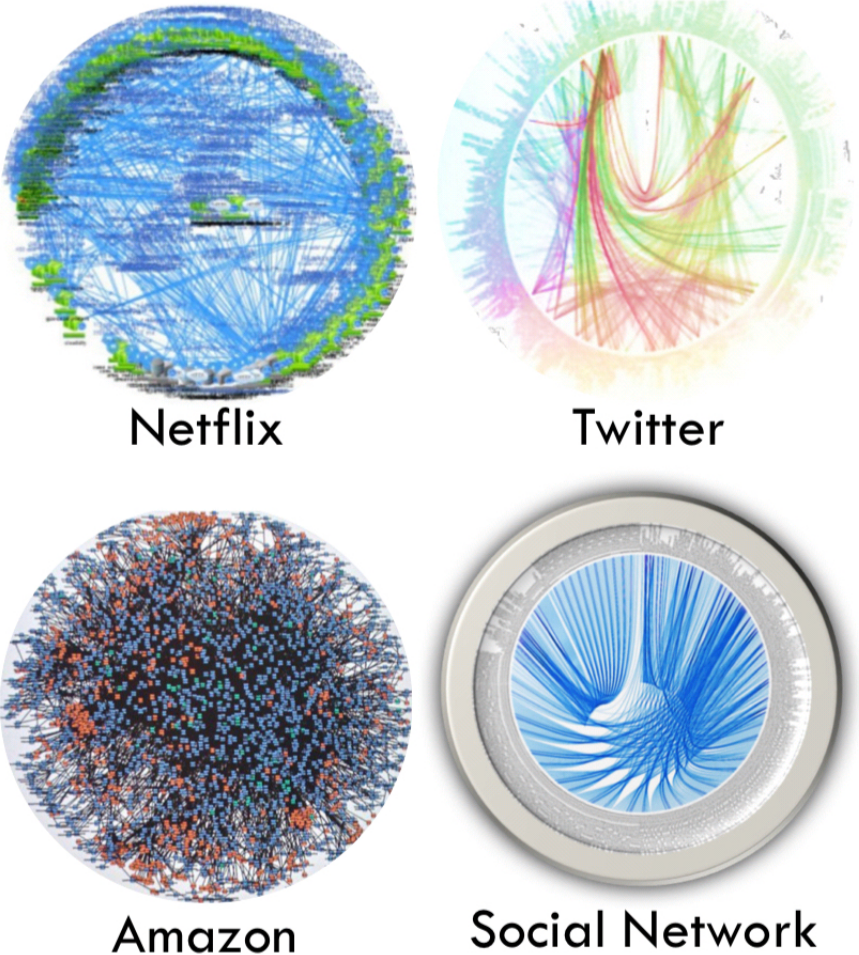
\includegraphics[width=1\linewidth]{Figures/large-scale-microservices.png}      
    \end{column}
    \begin{column}{.5\linewidth}
      \begin{itemize}
        \item Explosion de services
        \item Comment comprendre ? Comment déboguer ?
        \item Tous les services sont-ils essentiels ?
      \end{itemize}   
    \end{column}
  \end{columns} 
\end{frame}

\begin{frame}{Contenu supplémentaire}

\begin{itemize}
  \item Support de Thomas ROPARS et Renaud LACHAIZE
  \begin{itemize}
    \item \url{https://m2-mosig-cloud.gitlab.io/lectures/}
    \item \url{https://roparst.gricad-pages.univ-grenoble-alpes.fr/cloud-tutorials/m2gi-devops/}
  \end{itemize}
  \item Qu'est-ce que le concept de "cloud natif" ? : \url{https://cloud.google.com/learn/what-is-cloud-native?hl=fr}
  \item What Are Microservices : \url{https://youtu.be/CdBtNQZH8a4}
  \item Microservices : \url{https://martinfowler.com/articles/microservices.html}
  \item Newman, Sam. Building microservices. "O'Reilly Media, Inc.", 2021.
  \item Burns, Brendan. Designing distributed systems: patterns and paradigms
  for scalable, reliable services. "O'Reilly Media, Inc.", 2018.
\end{itemize}
  
\end{frame}


\end{document}